\chapter{那些好用的键盘快捷键}
\label{cha:shortcut-keys}

\begin{intro}
  相信大家对「快捷键」早已不陌生。这一节我们要介绍的快捷键,并不是像 \keys{Ctrl + C} 「复制」,\keys{Ctrl + V} 「粘贴」这样的我们早已耳熟能详的常用快捷键,而是那些很多新手未必一定知道但十分好用的快捷键和键盘用法。
\end{intro}

在开始之前,如果你不知道类似 \keys{Ctrl + Shift + S} 的快捷键怎么按,请参阅\chapref{cha:first-things-first}。

这部分其实更像一个「快捷键列表」,并不建议大家全部记住并使用。相反,你可以看一条尝试一条,然后渐渐地在日常使用和工作中去使用那些你觉得顺手的快捷键。有言曰:「习惯成自然。」

\section{\texorpdfstring{\keys{\protect\Windows\hspace*{.15em}} 键相关}{Windows 键相关}}

\keys{\Windows} 键是键盘上印有 Windows 徽标(形如 \Windows{} 或 \WindowsTen)的那个键,一般位于左 \keys{Ctrl} 键和左 \keys{Alt} 键之间。与 \keys{\Windows} 键有关的这些快捷键都是 Windows 系统级的快捷键。

\begin{itemize}
  \item \keys{\Windows + Shift + S}:在 Windows 10 和 Windows 11 中划区截屏。截屏结束后自动复制图片,若点击之后右下角弹出的通知还可以进一步进行简单的编辑。\CJKsout*{很多人不知道这个快捷键时,为了截屏专门打开 QQ 或微信。}
  \item \keys{\Windows + D}:最小化当前打开的所有窗口,然后返回桌面;如果再按一次,会恢复被最小化的那些窗口。
  \item \keys{\Windows + E}:打开「文件资源管理器」。当你想快速打开某个文件时,按这个快捷键比返回桌面双击「此电脑」要来得更快。
  \item \keys{\Windows + I}:在 Windows 10 和 Windows 11 中用来快速打开系统设置。
  \item \keys{\Windows + L}:锁屏。锁屏后需要输入密码才能解锁,这个快捷键适用于你需要短时间离开电脑而不希望别人看到你正在进行的工作时。
  \item \keys{\Windows + P}:投影。当你需要连接到投影仪时,你可以用它来选择不同的投影选项。
  \item \keys{\Windows + V}:在 Windows 10 和 11 中打开剪切板历史,可以看到你之前复制过的一系列内容。
  \item \keys{\Windows + X}:在 Windows 10 和 11 中打开「开始右键菜单」(有时也被称作「超级用户菜单」,就是在开始按钮右击所弹出的菜单),可以快速打开一些系统组件。
  \item \keys{\Windows + ;}:在 Windows 10 和 11 中打开 emoji 面板,可以快速查找并输入 emoji。
  \item \keys{\Windows + Pause} 或 \keys{Break}\footnote{一般说来,\keys{Pause} 和 \keys{Break} 键在键盘的右上角,但一些键数比较少的键盘以及笔记本电脑键盘可能没有 \keys{Pause} 或者 \keys{Break} 键。}:快速打开「系统信息」页面,可以很方便地从此前往「高级系统设置」。
  \item \keys{\Windows} + 方向键:
  \begin{itemize}
    \item \keys{\Windows + ↑}:最大化当前窗口;如果已经最大化了,再按会让窗口向上吸附。
    \item \keys{\Windows + ↓}:缩小当前窗口;如果已经是缩小的了,再按会让窗口最小化。
    \item \keys{\Windows + ←} 和 \keys{\Windows + →}:左右吸附当前窗口。当窗口吸附到一侧时,按另一侧的吸附快捷键就能还原。
  \end{itemize}

  先后按下这些快捷键组合中的几个,说不定能够将你的几个窗口吸附到屏幕的四个角落,就像这样:

  \begin{figure}[htb!]
    \centering
    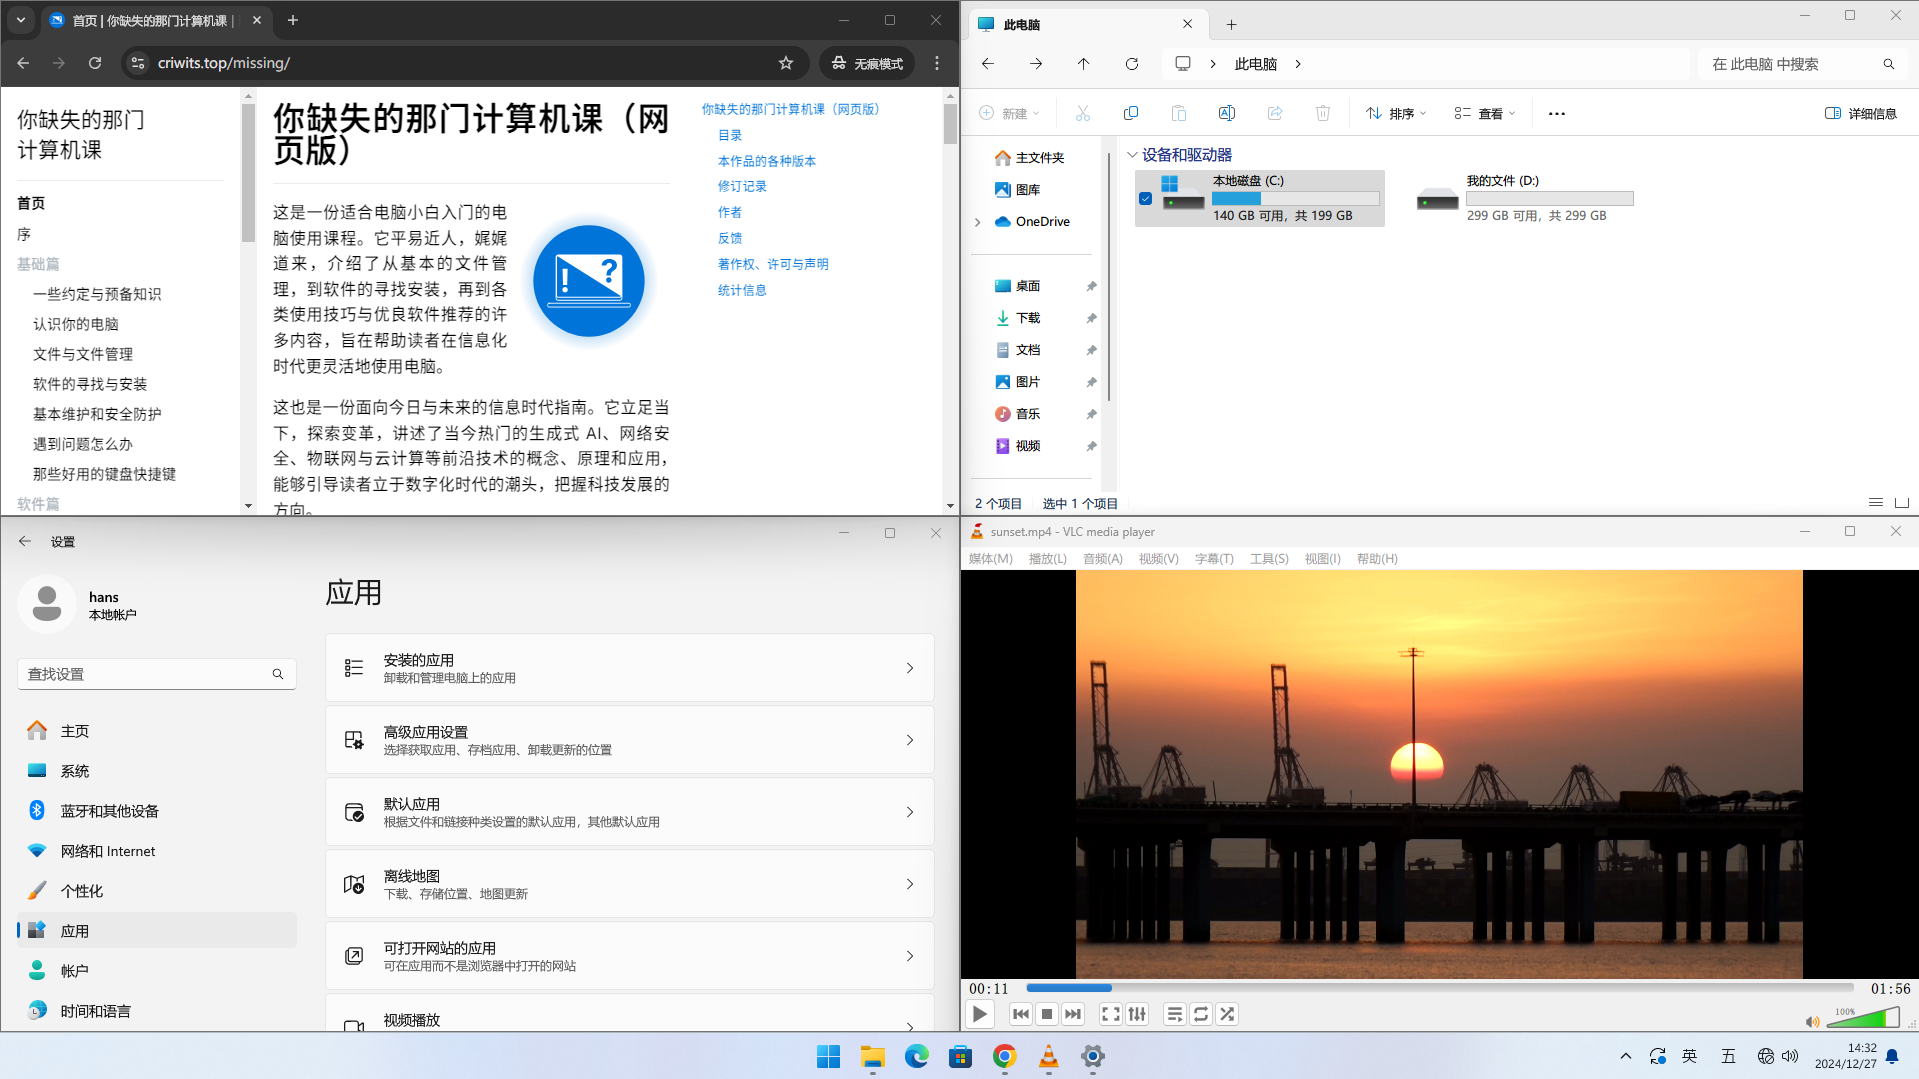
\includegraphics[width=.7\textwidth]{assets/basic/Window_Grid.png}
    \caption{屏幕四角的窗口们}
    \label{fig:Window_Grid}
  \end{figure}

  \item 「虚拟桌面」相关:

  「虚拟桌面」是自 Windows 10 以来微软\CJKsout*{抄来的}推出的一种新的窗口管理方式。借助虚拟桌面,你可以在一台电脑上获得多个屏幕的使用体验。
  \begin{itemize}
    \item 按 \keys{\Windows + Tab},你可以看到一个【新建桌面】的按钮。Windows 10 的这个按钮位于画面顶部,Windows 11 则在底部。按这个按钮,你原来打开的应用全部留在「桌面 1」,而一个新的虚拟桌面「桌面 2」则会呈现在你面前。桌面 1 上的应用全部继续工作,而在桌面 2 上,你亦可以打开一些新的应用,干一些其他的事情。下图展示的是 Windows 11 下的两个虚拟桌面:
      \begin{figure}[htb!]
        \centering
        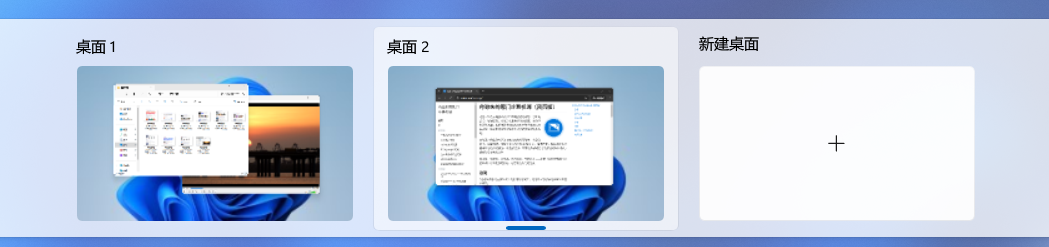
\includegraphics[width=.85\textwidth]{assets/basic/Virtual_desktop.png}
        \caption{两个虚拟桌面}
        \label{fig:Virtual_desktop}
      \end{figure}
    \item 在 \keys{\Windows + Tab} 中,你可以在两个桌面间切换。    
    \item \keys{\Windows + Ctrl + D} 可以用来创建一个新的虚拟桌面,这等价于按 \keys{\Windows + Tab} 然后手动点击【新建桌面】按钮。
    \item \keys{\Windows + Ctrl + ←} 和 \keys{→} 可以在多个虚拟桌面间切换,这等价于按 \keys{\Windows + Tab} 然后手动点选不同的虚拟桌面。
  \end{itemize}
\end{itemize}

\section{\keys{Ctrl} 键相关}

这里介绍的与 \keys{Ctrl} 有关的快捷键中,一些是系统级的快捷键,在系统的任何地方都能使用;另一些是软件内提供的快捷键,不过它们的用法都已约定俗成,因而在不同软件中都有着相同的功能。

\begin{itemize}
  \item \keys{Ctrl + A}:全选。在文件管理器中,按这个快捷键可以全选所有的文件和文件夹;而在编辑文本时,它可以选中当前输入框内所有的文本。例如,当你在 QQ 中想删掉已经打出来的所有内容时,只需按一次 \keys{Ctrl + A},再按 \keys{Backspace} 就能完成这个操作。
  \item \keys{Ctrl + D}:删除文件。仅适用于资源管理器,相当于按一次 \keys{Delete}。
  \item \keys{Ctrl + F}:搜索。这个快捷键适用于大多数文本编辑器,例如「记事本」或 Word。按这个快捷键可以调出文本搜索的对话框。
  \item \keys{Ctrl + H}:替换。同上,这个快捷键适用于大多数文本编辑器,可以调出文本替换的对话框。
  \item \keys{Ctrl + Z}:撤销。这个快捷键适用于大多数工作软件,作用是撤销上一步操作。
  \item \keys{Ctrl + Y}:恢复。同上,这个快捷键适用于大多数工作软件,作用是恢复上一步撤销的操作。
  
  但如果你发现这玩意不是恢复的话,不妨试试 \keys{Ctrl + Alt + Z} 或者 \keys{Ctrl + Shift + Z},这些或许才是当前软件的「恢复」快捷键。

  \item 适用于大多数富文本\footnote{富文本(rich text)又称「格式化文本」,指具有风格、排版等信息的文本。}编辑器(例如 Word、WPS 和 Obsidian)的文本样式快捷键:
  \begin{itemize}
    \item \keys{Ctrl + B}:加粗。
    \item \keys{Ctrl + I}:斜体。
    \item \keys{Ctrl + U}:下划线。
  \end{itemize}
  \item \keys{Ctrl + S}:保存。适用于绝大多数软件。
  \item \keys{Ctrl + Tab}:切换标签页。适用于大多数浏览器(标签页就是浏览器上方可以切换的多个页面)。
  \item \keys{Ctrl + W}:关闭当前打开的标签页。同上,适用于大多数浏览器。
  \item \keys{Ctrl + P}:打印。适用于大多数办公软件,例如 Word、PPT 和 Excel。
  \item \keys{Ctrl + 鼠标滚轮}:在浏览器、Office 等软件中用于缩放页面。按住 \keys{Ctrl} 并向上滚动可以放大页面,向下滚动则可以缩小页面。
  \item \keys{Ctrl + Alt + Z}:适用于 QQ/TIM。用来调出 QQ/TIM 的消息界面。
  \item \keys{Ctrl + Alt + W}:适用于微信。用来调出微信的消息界面。
\end{itemize}

\section{\keys{Alt} 键相关}

单独与 \keys{Alt} 键相关联的快捷键并不多,常用的有下面两个。

\begin{itemize}
  \item \keys{Alt + F4}:退出当前程序。例如,你现在按一下 \keys{Alt + F4} 大概会关闭本文档。如果你在桌面按下它,就会弹出【关闭 Windows】的窗口。
  \item \keys{Alt + Tab}:在当前打开的各个应用中切换。这个快捷键的用法是这样的:先按住 \keys{Alt} 并保持,然后按一下 \keys{Tab},就可预览当前打开的所有应用。保持按住 \keys{Alt},每按一次 \keys{Tab} 就能选择界面中的下一个应用(若按住 \keys{Shift} 再按 \keys{Tab} 则选择上一个应用)。当你松开所有按键的时候,就会切换到最后被选中的那个应用上。

  如果按一次 \keys{Alt + Tab} 就松开所有按键,会切换到上一个使用过的应用上。

\end{itemize}

\practice

逐个尝试上面的快捷键,然后将那些你用得顺手的快捷键应用在你的工作、学习和生活中。
